% !TEX root = ../document.tex
% !TeX spellcheck = pt_BR

\section{O que é isquemia cardíaca?}

\begin{frame}{O que é isquemia cardíaca?}
    Do grego:
    \hskip10pt \alert{iskhein} $+$ \alert{haima} $=$ constrição sanguínea\\
    \hskip55pt restringir\hskip10pt sangue
    \vskip20pt
    \begin{block}{\alert{Isquemia cardíaca}}
        É a redução ou falta de suprimento de sangue a uma região do músculo do coração (miocárdio).
    \end{block}
    \vskip20pt
    Pode causar infarto do miocárdio.
\end{frame}

\begin{frame}{O que é isquemia cardíaca?}
    \begin{center}
        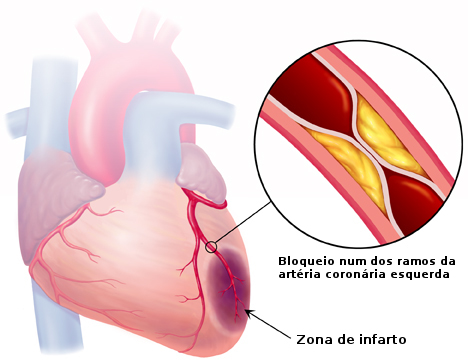
\includegraphics[scale=0.5]{figures/infarction.jpg}
    \end{center}
    \tiny Adaptado de:\\
    \url{http://nursingcrib.com/nursing-care-plan/nursing-care-plan-myocardial-infarction/}
\end{frame}